\documentclass{beamer}
\usetheme[compress]{Singapore}

\usepackage{scrextend} % For margins

\usepackage[english]{babel}		
\usepackage[utf8x]{inputenc}
\usepackage{microtype}
\usepackage{graphicx}
\usepackage{amsmath}
\usepackage{amssymb}
\usepackage{amsfonts}
\usepackage{mathtools}
\usepackage{siunitx}
\usepackage{xspace}
\usepackage{mathrsfs}
\usepackage{slashed}
%\usepackage[inline]{enumitem}
\usepackage{enumerate}
\usepackage{cleveref}
\usepackage{booktabs}
\usepackage{bbold}

\usepackage{subcaption}
\usepackage{caption}

\newcommand{\norm}[1]{\left\lVert#1\right\rVert}
\newcommand{\mb}[1]{\mathbf{#1}}

\title{Journal Club 7-12-2017}
\author{Malthe Kj\ae r Bisbo}


\begin{document}
\begin{frame}
	\titlepage
\end{frame}

\begin{frame}{Articles}
	\begin{block}{Article 1}
		\textit{Sampling Polymorphs of Ionic Solids using Random Superlattices}
	\end{block}
	\begin{block}{Article 2}
		\textit{Ab initio random structure search}
	\end{block}
\end{frame}

\begin{frame}{Article 1}
\begin{block}{"Packing" Polymorphs}
	Solids with similar stoichiometry  but different crystal structure/packing.
\end{block}
\begin{columns}
	\column{0.5\textwidth}
	Polymorphs are found at the bottom of funnels
	
	\column{0.5\textwidth}
	\begin{figure}
		\centering
		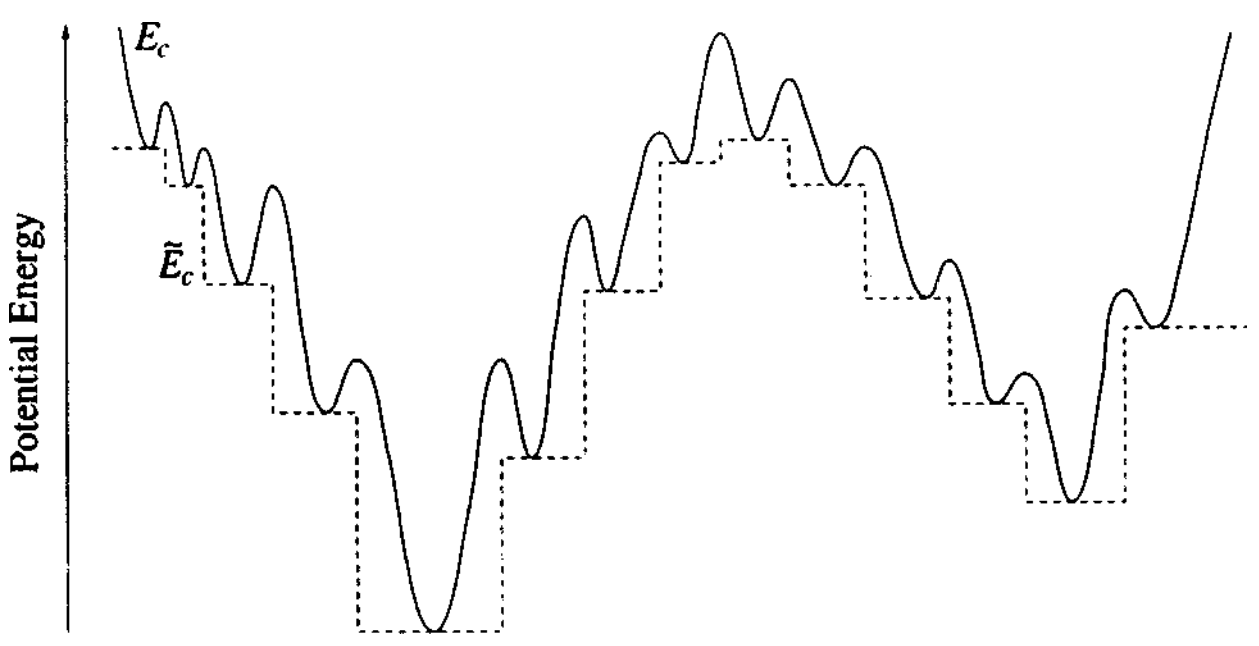
\includegraphics[width=0.9\linewidth]{Funnel_of_basins}
		\caption{Two funnels containing multiple basins}
		\label{fig:funnelofbasins}
	\end{figure}
\end{columns}
\end{frame}

\begin{frame}{Article 1}
\begin{block}{Factors influencing realizability of polymorphs}
	\begin{enumerate}
		\item Energy above ground state
		\item Energy barrier to escape minimum
		\item Volume of configuration space occupied by the minimum of the polymorph.
	\end{enumerate}
\end{block}
This article focuses on assigning configuration space volumes.
\bigskip

The third factor might be a simplification as the volume of the whole funnel will probably contribute to the minimum basin of the funnel.
\end{frame}

\begin{frame}{Article 1}
\begin{block}{Sampling using Random Superlatices}
\begin{figure}
	\centering
	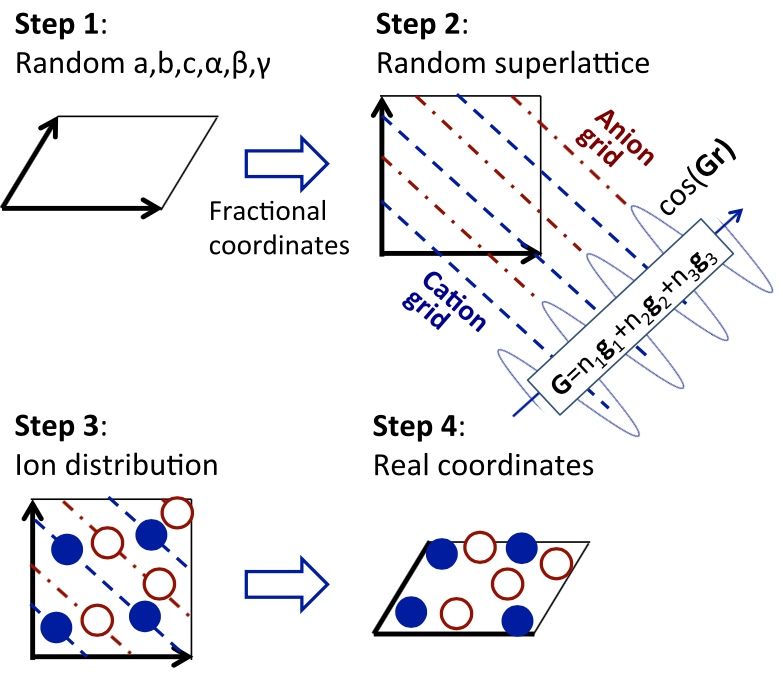
\includegraphics[width=0.5\linewidth]{SuperlatticeSampling}
	\label{fig:superlatticesampling}
\end{figure}

\end{block}
\end{frame}

\begin{frame}{Article 2}
\begin{block}{Complexity of PES - motivational argument}
	\begin{enumerate}
		\item Consider deviding a system of N atoms into M subsystems.
		\item Assume that the M subsystems are large enough to have independent stable configurations.
		\item Neglecting changes in the number of stable configurations arising from combining the M sub systems.
	\end{enumerate}
	The total number of stable configurations $n_s(N)$ must then satisfy 
	\begin{align*}
	n_s(N) = \left(n_s(N/M)\right)^M
	\end{align*}
	with solution
	\begin{align*}
	n_s(N) = \exp^{\alpha N}
	\end{align*}
\end{block}
\end{frame}

\begin{frame}{Article 2}
\begin{block}{General remarks on the PES}
	\begin{enumerate}
		\item Almost no minima when atoms are close
		\item The barrier to lower lying minima are smaller than those to higher lying minima
		\item Low energy basins come in groups
		\item Low energy basins occupy larger configuration space volumes
	\end{enumerate}
	\begin{columns}
		\column{0.5\textwidth}
		The distribution of number of transitions connecting a minima has a power law tail.
		\bigskip
		The low energy minima are highly connected.
		
		\column{0.5\textwidth}
		\begin{figure}
			\centering
			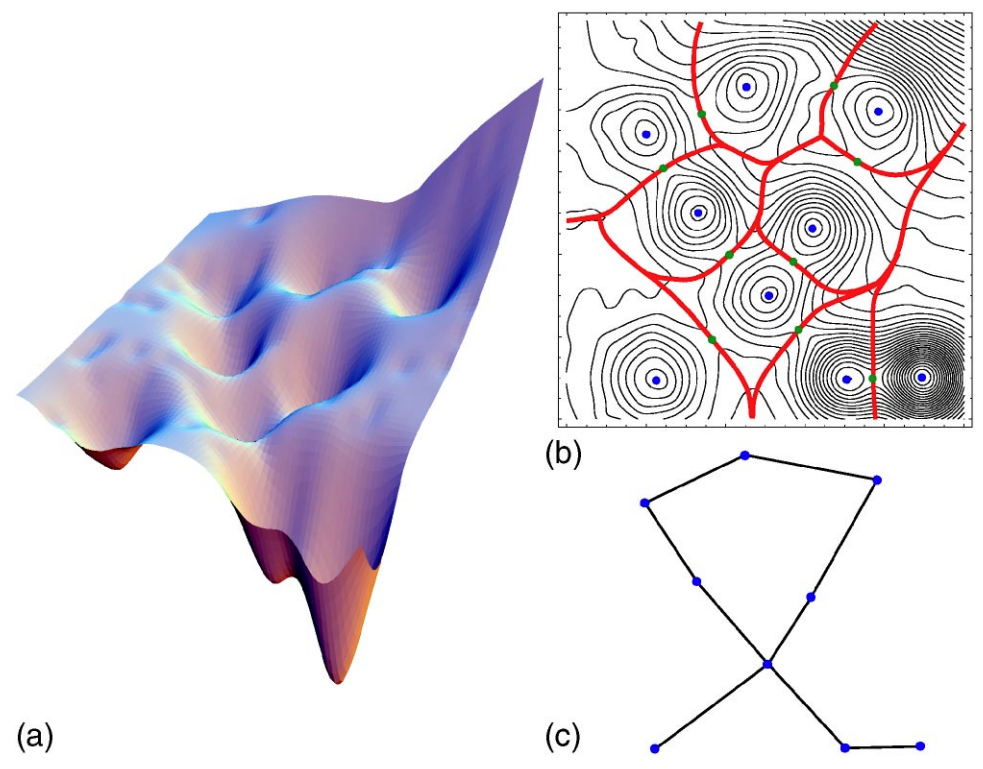
\includegraphics[width=0.9\linewidth]{PESasNetwork}
			\caption{}
			\label{fig:pesasnetwork}
		\end{figure}
		
	\end{columns}
\end{block}
\end{frame}

\begin{frame}{t-SNE}
\begin{itemize}
	\item Nonlinear dimensionality reduction 
	\item Maps points such that similar points remain close in the reduced space.
	\item Uses: Mapping to 2 or 3 dimensions, visualizing neural network representations.
\end{itemize}

\begin{block}{Investigation of the PES}
	\begin{itemize}
	\item DFT vs. DFTB+ 
	\item PES of molecules vs. solids
\end{itemize}
\end{block}

\end{frame}
\end{document}